\section {Motivation}

Node-aware all-to-all is a traditional method to optimize small message all-to-all.
Node-aware all-to-all will aggregate messages between each pair of node to reduce message number.

As shown in Figure ~\ref{Node-aware-alltoall}.
\begin{figure}[!htb]
  \centering
    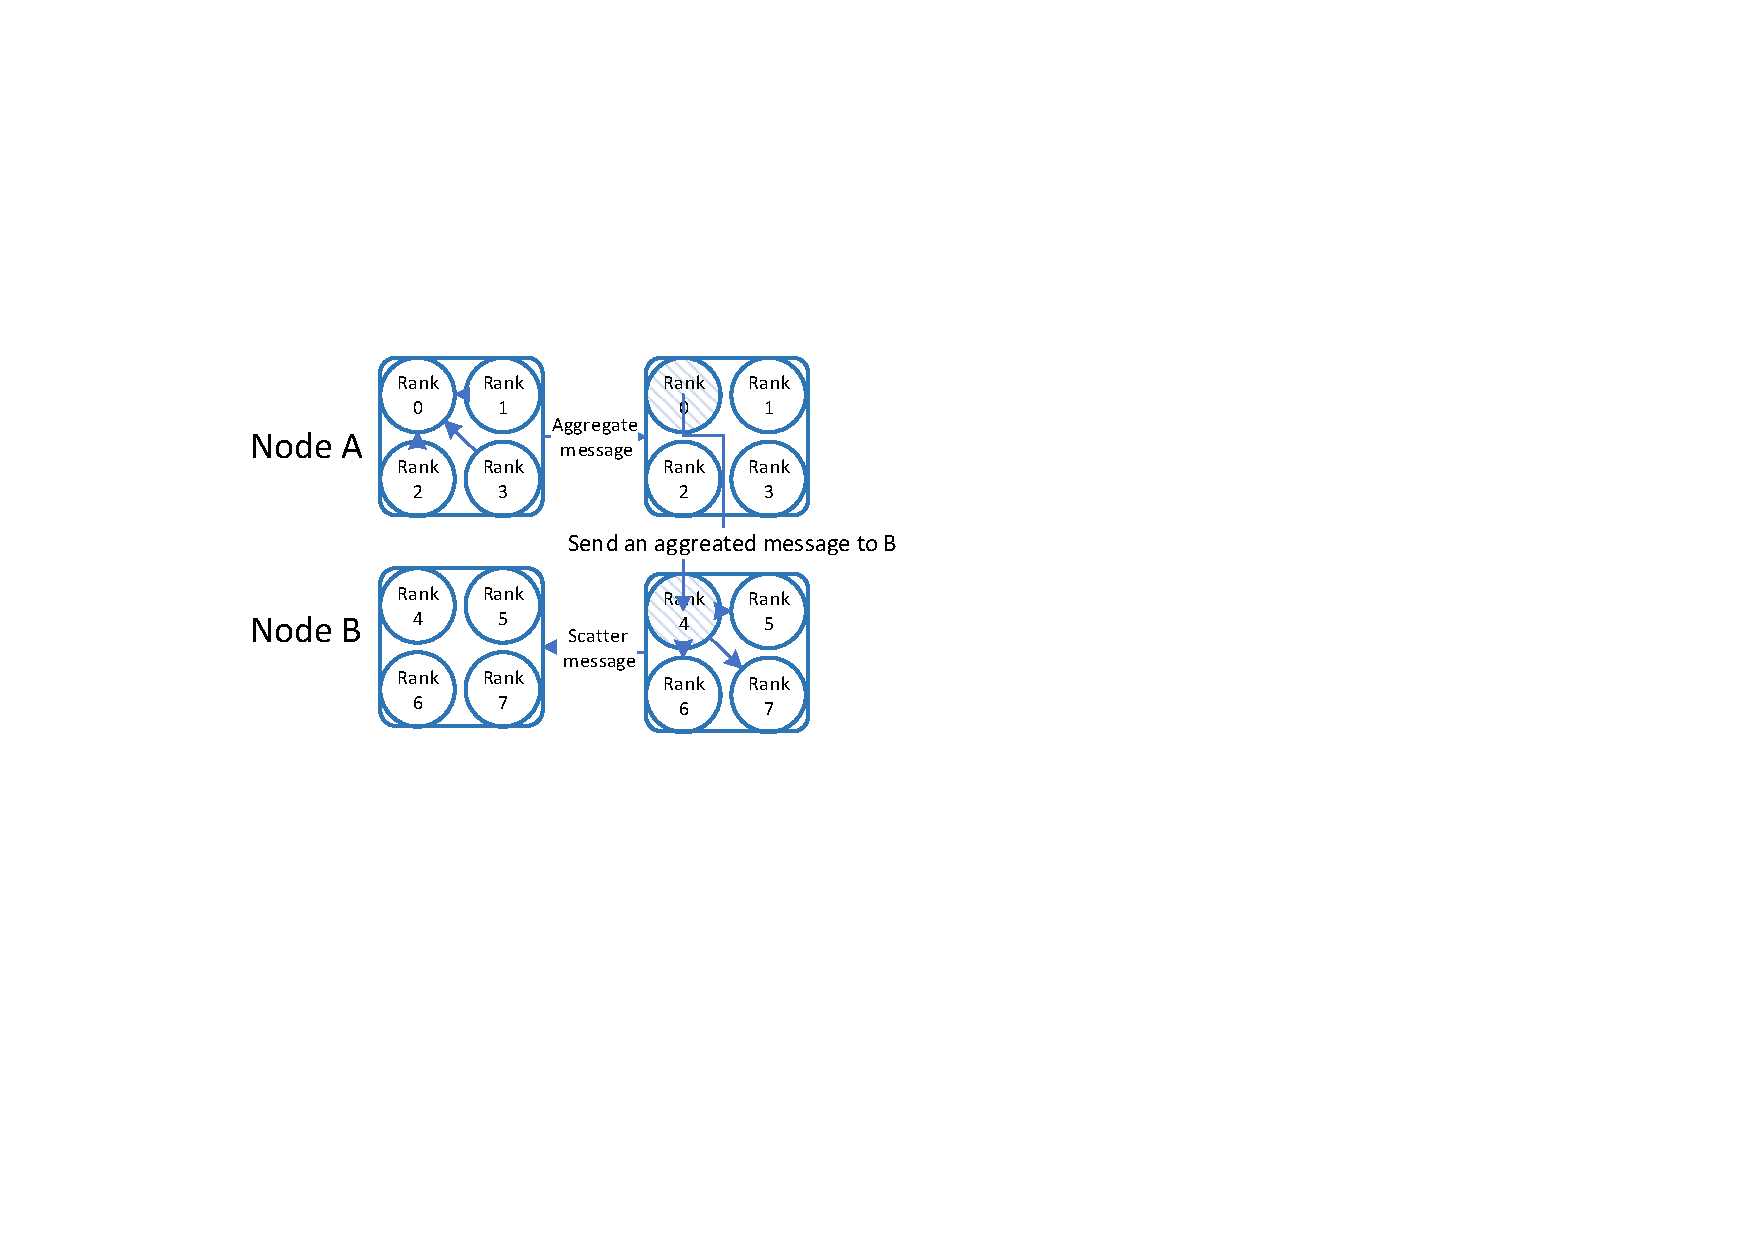
\includegraphics[width=0.49\textwidth]{./Figures/Node-aware-alltoall.pdf}
  \caption{Multi-leader gahtering/scattering throughput based on MPI-RMA, Leader Number $\in$ [1,2,4,8]}
	\label{Node-aware-alltoall}
	\vspace{0.2in}
\end{figure}

It include four steps: intra-node gather, local transpose, inter-node all-to-all, intra-node scatter.
For a 32/64 cores CPU, each inter-node message in node-aware method will be 1024/4096 times larger than direct method.
After aggreatation, the small messages become large messages and message number is reduced.
However, when message getting larger, gatering, transpose, and scattering overhead increase with the message size.
It limit the application scope of node-aware all-to-all.

With the increase in the number of processor cores, multiple CPU cores, NUMA, network endpoints and inter-/intra-node overlapping brings huge parallelism.
We notice that all traditional method do not take advantage of this parallelism to solve the problem.
As the single-core memory access bandwidth may not faster than the network bandwidth.
Using a single core to gather, scatter, and transpose data, and initialize communication request may causing communication hotspot on a CPU core.

Multi-leader can get faster message aggregation throughput than one-leader gathering/scattering.
Results of figure \ref{multileader-gather} show the multi-leader gathering/scattering throughput compared to one-leader.
\begin{figure*}[!htb]
  \centering
    \subfigure[HPC-A]{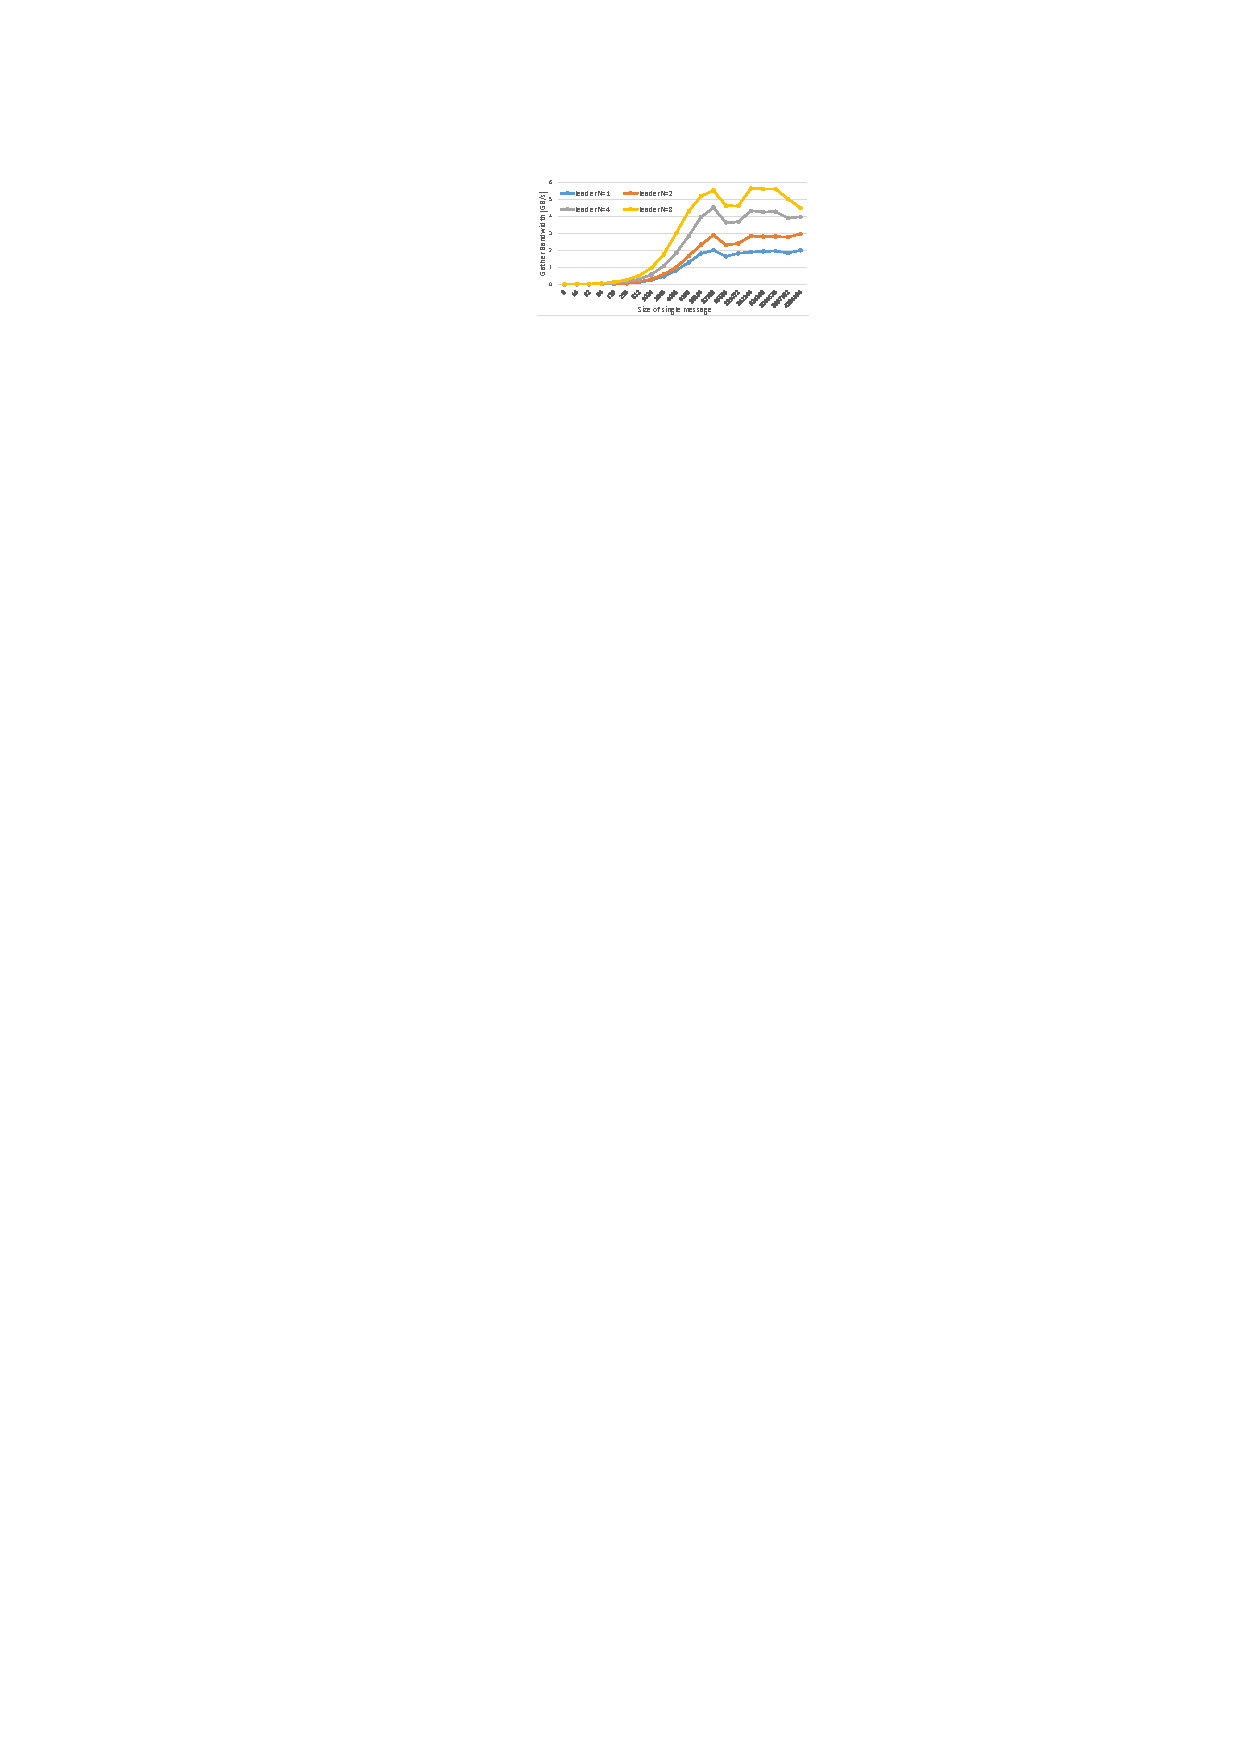
\includegraphics[width=0.49\textwidth]{./Figures/hpca/HPC-multi-leader-gather.pdf}}
	\subfigure[HPC-B]{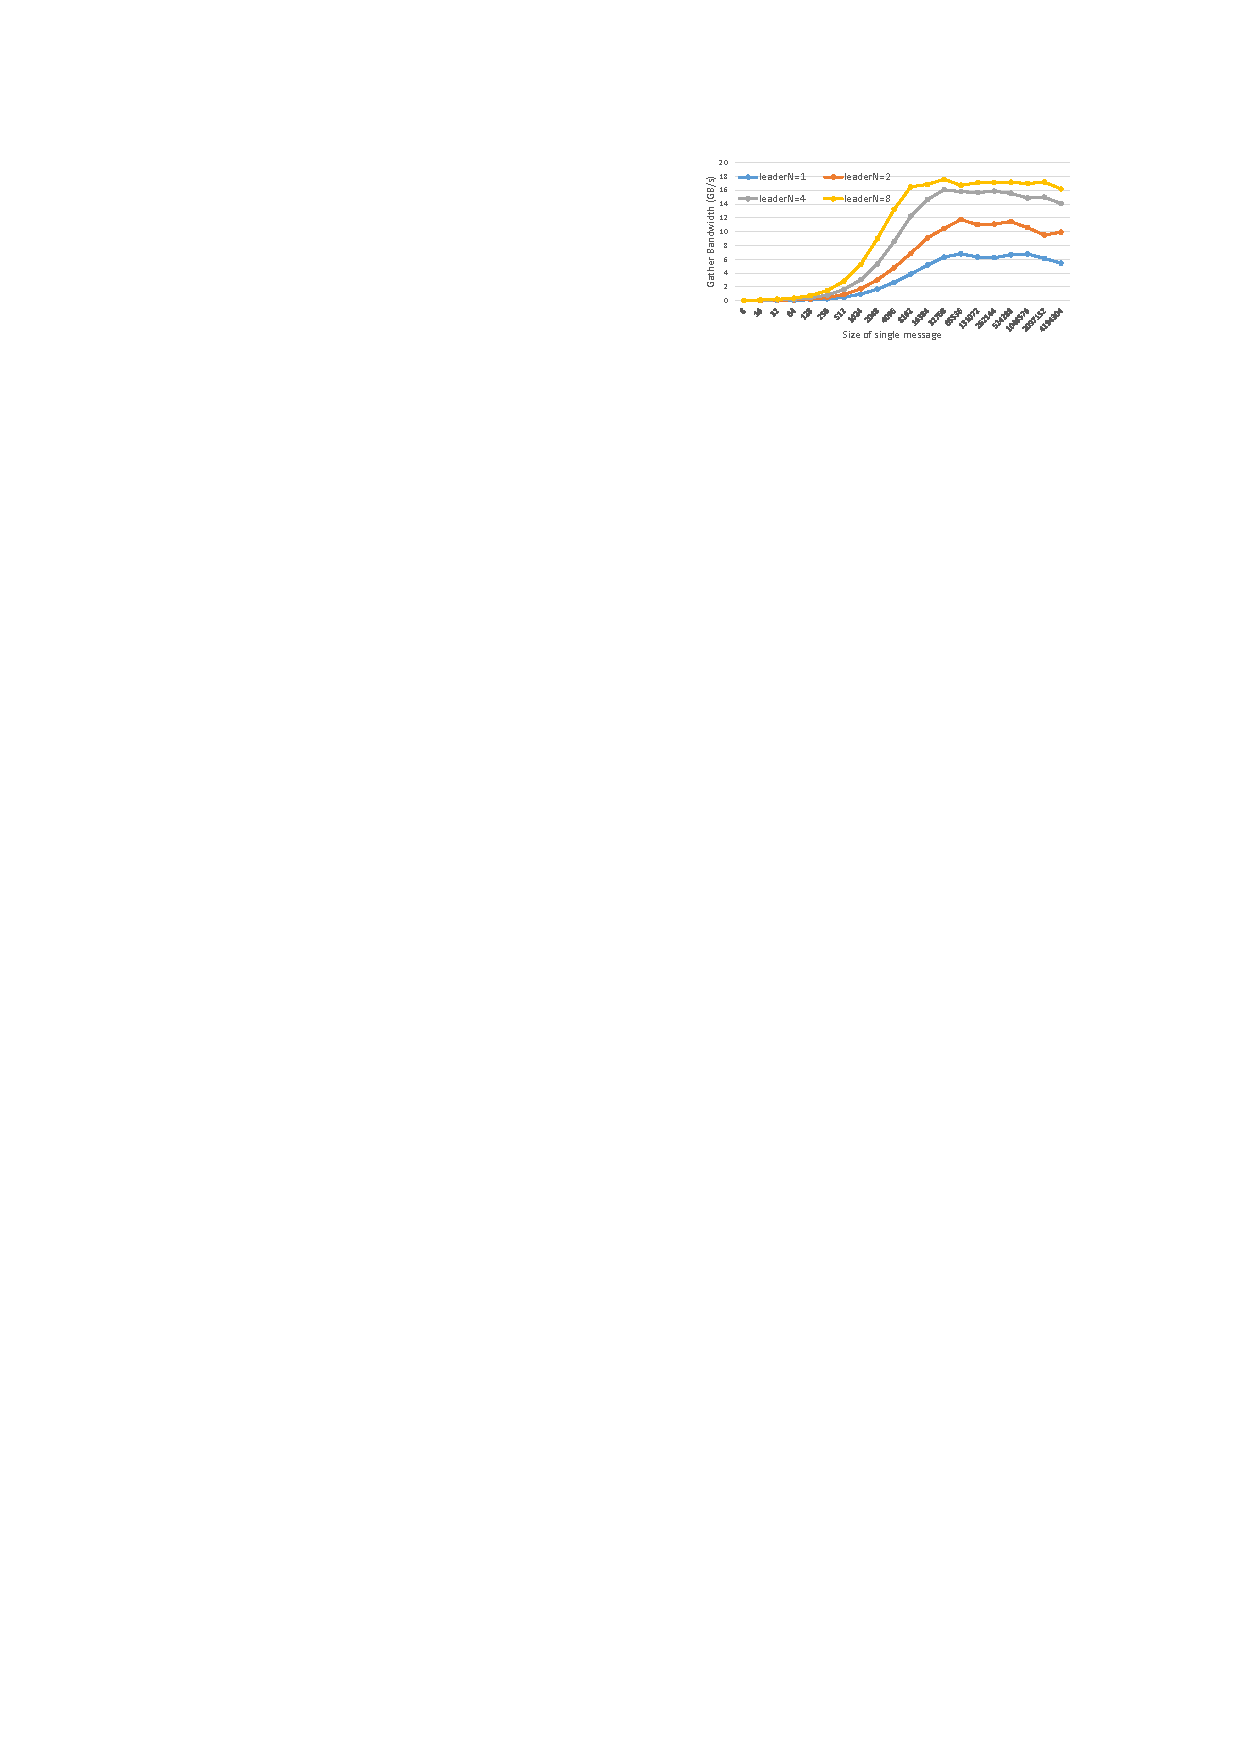
\includegraphics[width=0.49\textwidth]{./Figures/hpcd/HPC-multi-leader-gather.pdf}}
  \caption{Multi-leader gahtering/scattering throughput based on MPI-RMA, Leader Number $\in$ [1,2,4,8]}
	\label{multileader-gather}
	\vspace{0.2in}
\end{figure*}
Notice the result of HPC-B, its one-leader gathering/scattering bandwidth is about 6 GB/s, while it p2p bandwidth is 7.089 GB/s.
As a node-aware all-to-all includes: intra-node gather, inter-node all-to-all, intra-node scatter steps.
The overhead to aggregate M gigabyte messages is about M/6 second.
The overhead to send it to another node is about M/7 second.
The overhead to scatter it on is about M/6 second.
In this case, intra-node communication become  bottelneck of node-aware all-to-all.
Using multiple leaders can improve the gathering and scattering thoughput on a node.

With non-uniform memory access (NUMA) systems has emerged, a CPU is composed with multi-socket. 
When different core try to access a same NUMA, its local memory bandwidth is shared between multiple cores.
For a Multi-leader gathering/scattering on these processors, NUMA architecture has performance effect on gathering/scattering performance. 
Putting multiple leader on the same NUMA or lets leaders uniform distributed on the CPU may have significant performance difference.
We bind each processes to corresponding core and compared the NUMA-aware and test the NUMA-aware multi-leader gahtering/scattering  Vs multi-leader gahtering/scattering.
The performance improvements are shown in Figure \ref{UMA-aware-multi-leader}.
Because the CPU has multiple memory access units for different NUMAs.
\begin{figure*}[!htb]
  \centering
    \subfigure[HPC-A 4 NUMAs in a node]{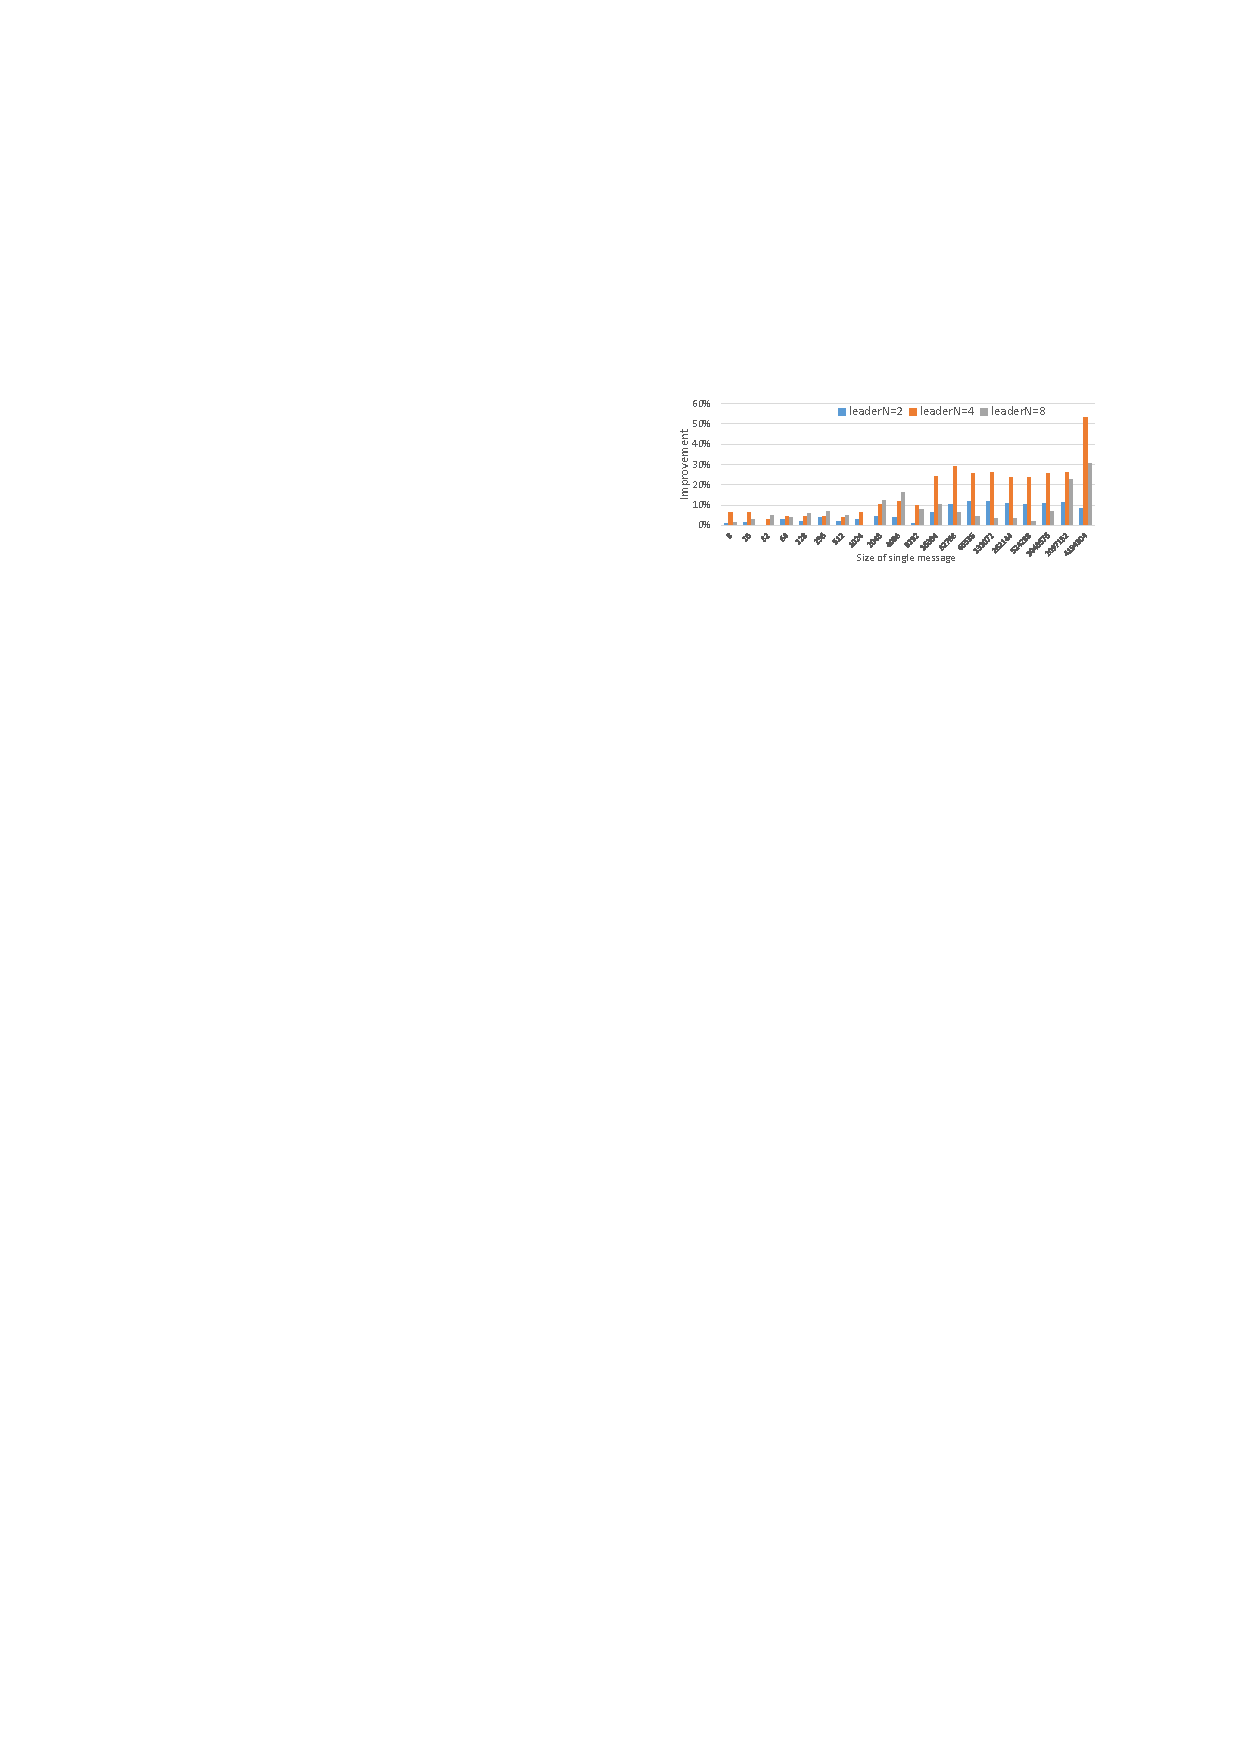
\includegraphics[width=0.49\textwidth]{./Figures/hpca/NUMA-aware-gather-scatter.pdf}}
	\subfigure[HPC-B 2 NUMAs in a node]{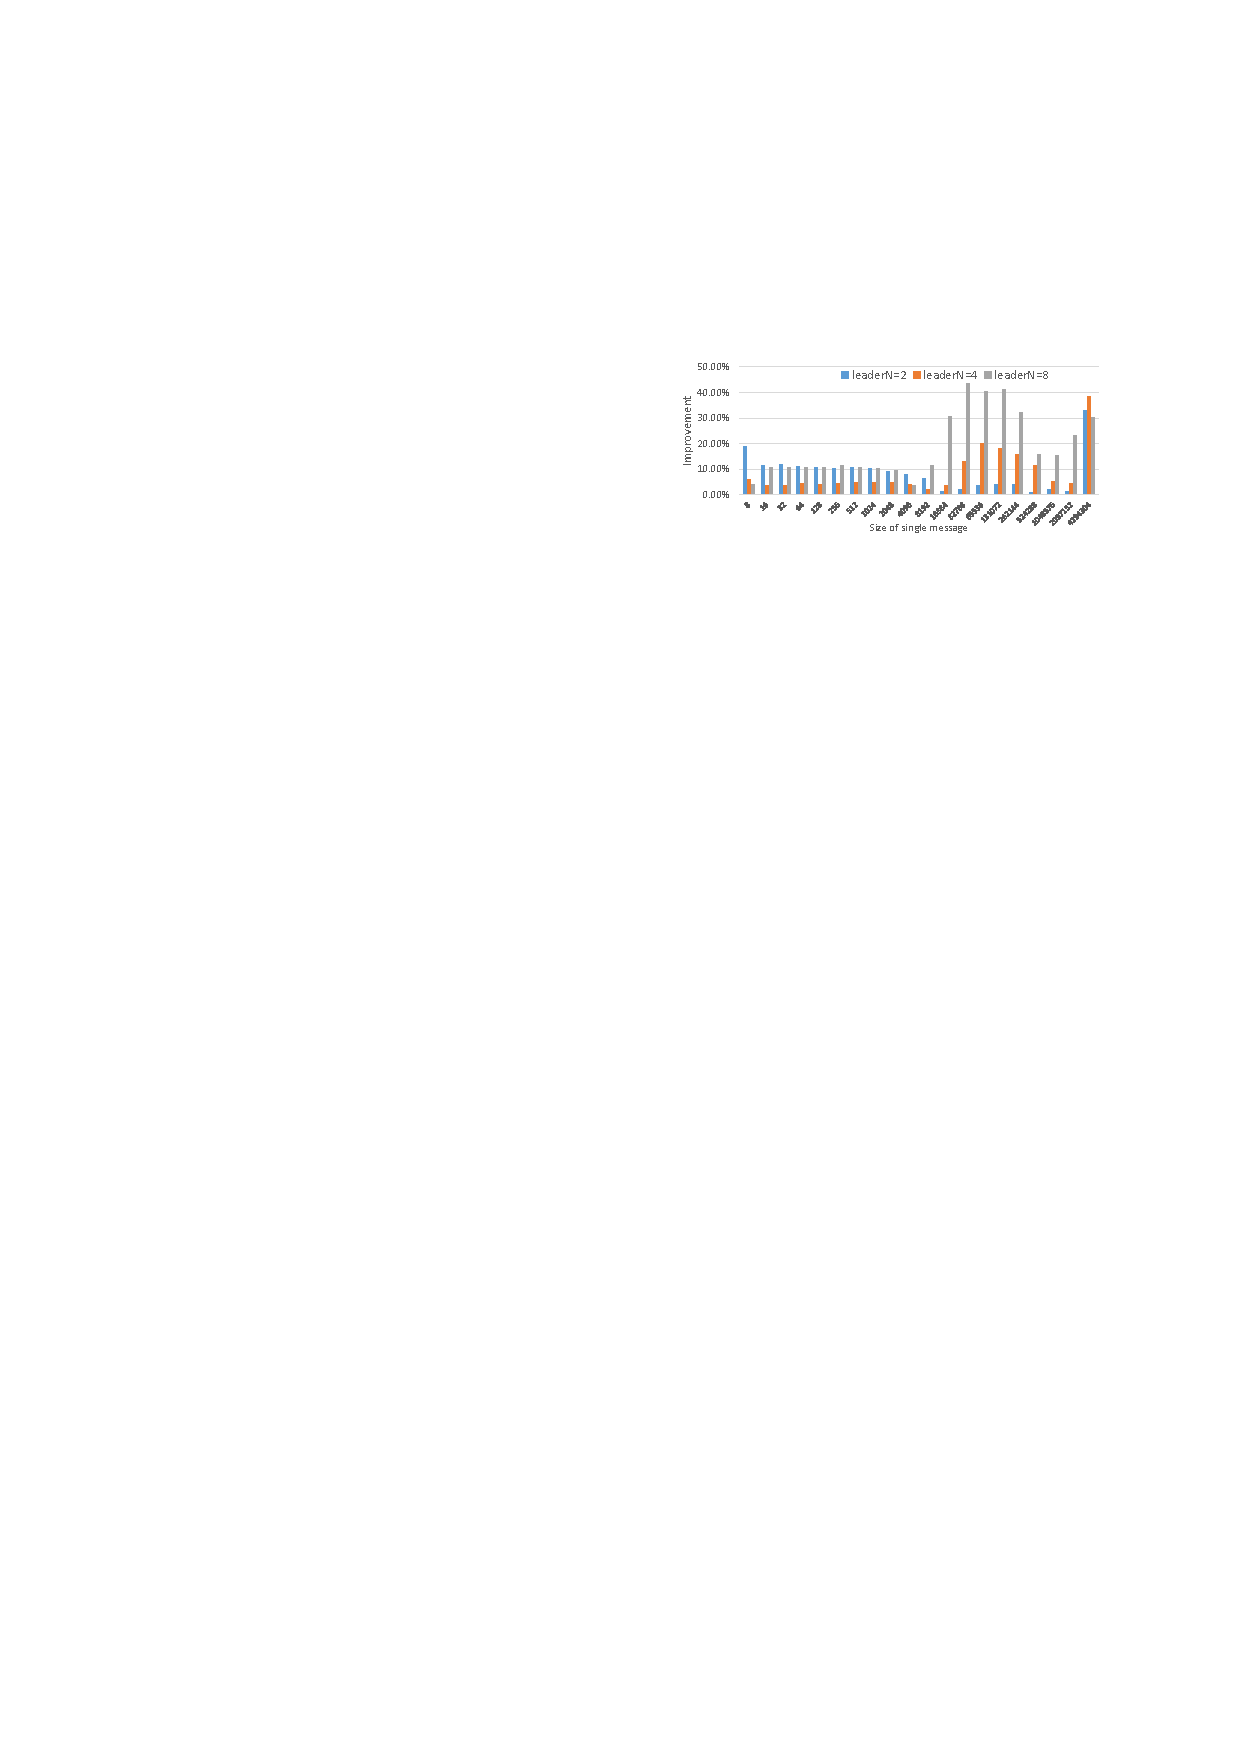
\includegraphics[width=0.49\textwidth]{./Figures/hpcd/NUMA-aware-gather-scatter.pdf}}
  \caption{NUMA-aware multi-leader gahtering/scattering throughput compared to multi-leader gahtering/scattering.}
	\label{NUMA-aware-multi-leader}
	\vspace{0.2in}
\end{figure*}

Morden interconnect network on supercomputer usually have multiple endpoints for each nodes.
Multiple endpoints improve the concurrent ability to process multiple communication requests.
We uses two nodes, one nodes activate several processes to concurrently send to corresponding processes on another node.
As each process in a nodes will activate a network endpoints, the number of activated processes number in a node is equal to the number of network endpoint in using.
As Figure \ref{Multi-port} show, we find that multiple endpoints do improve the node-to-node throughput in most cases.
\begin{figure*}[!htb]
  \centering
    \subfigure[HPC-A 4 NUMAs in a node]{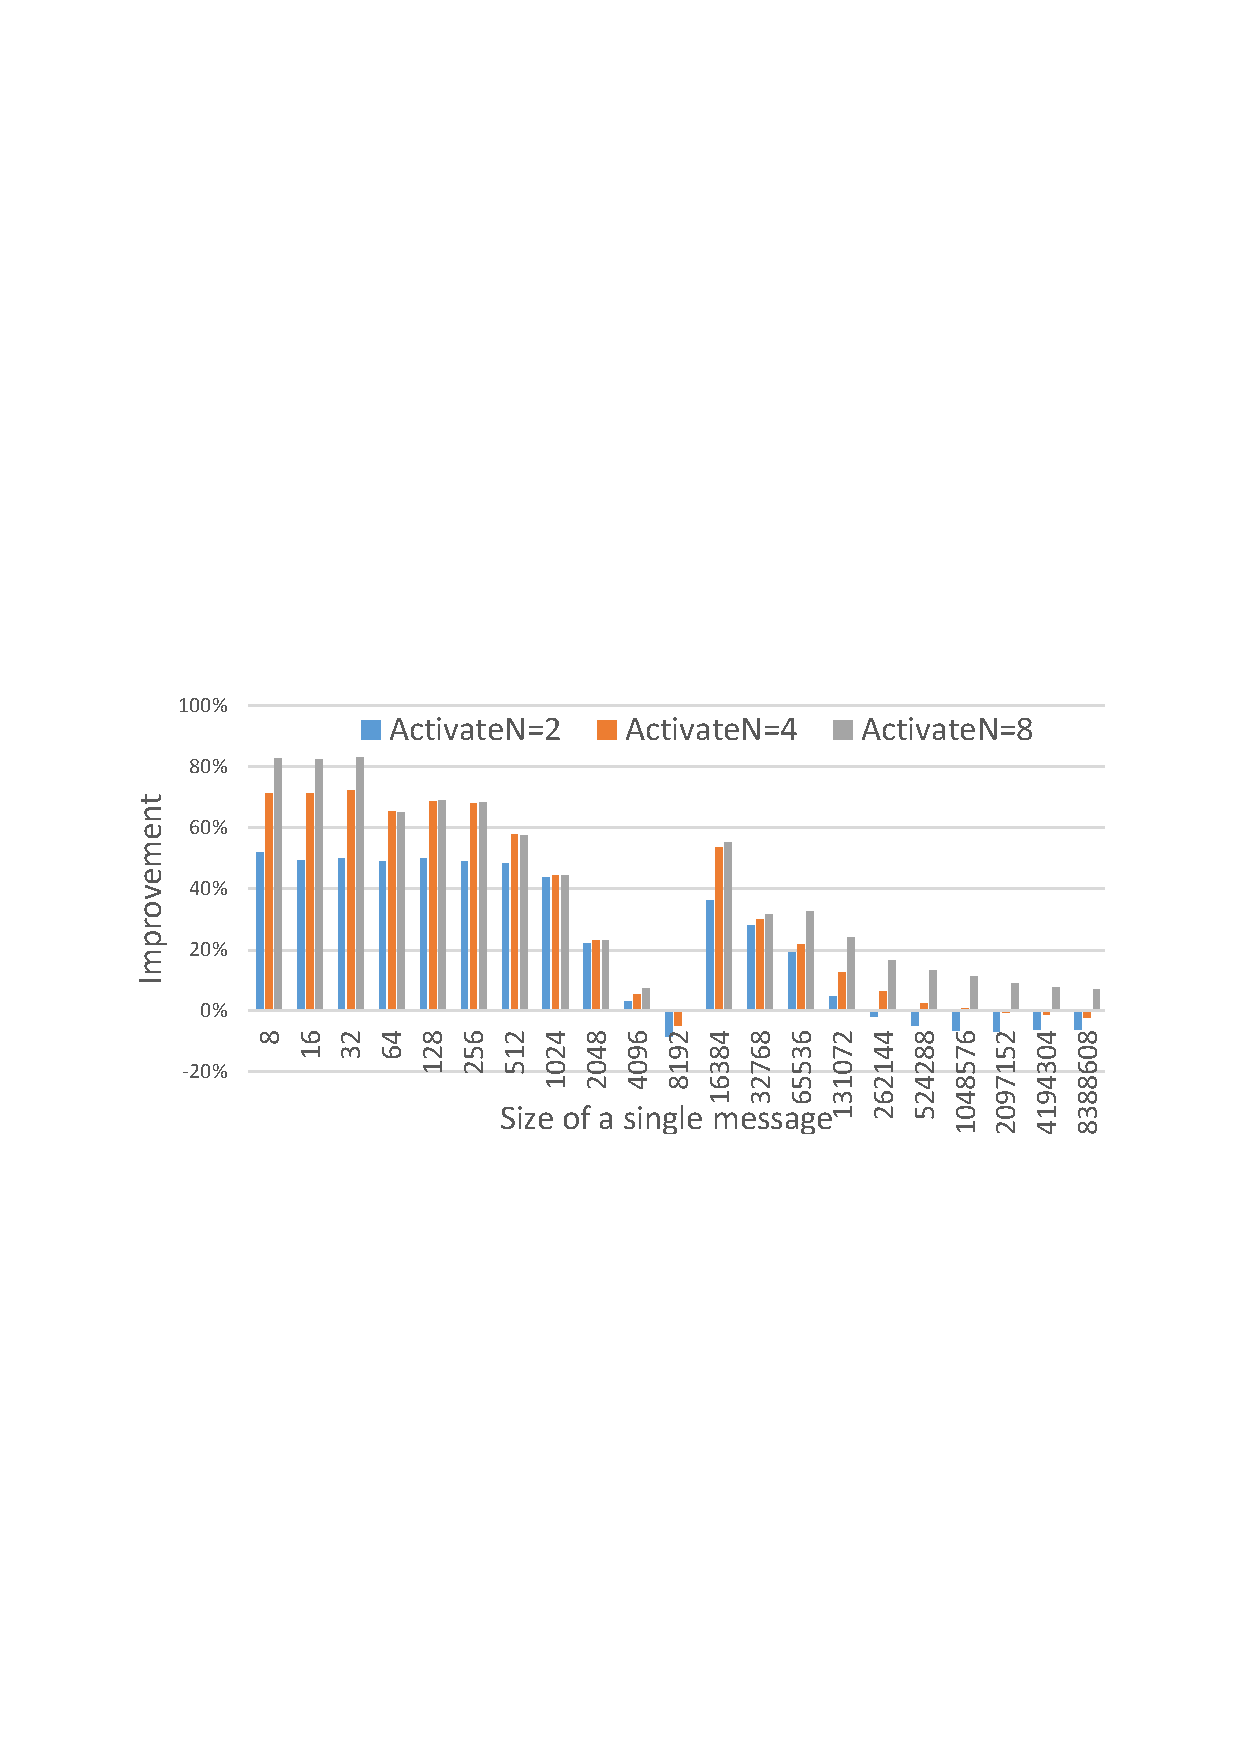
\includegraphics[width=0.49\textwidth]{./Figures/hpca/Multi-port-p2p.pdf}}
	\subfigure[HPC-B 2 NUMAs in a node]{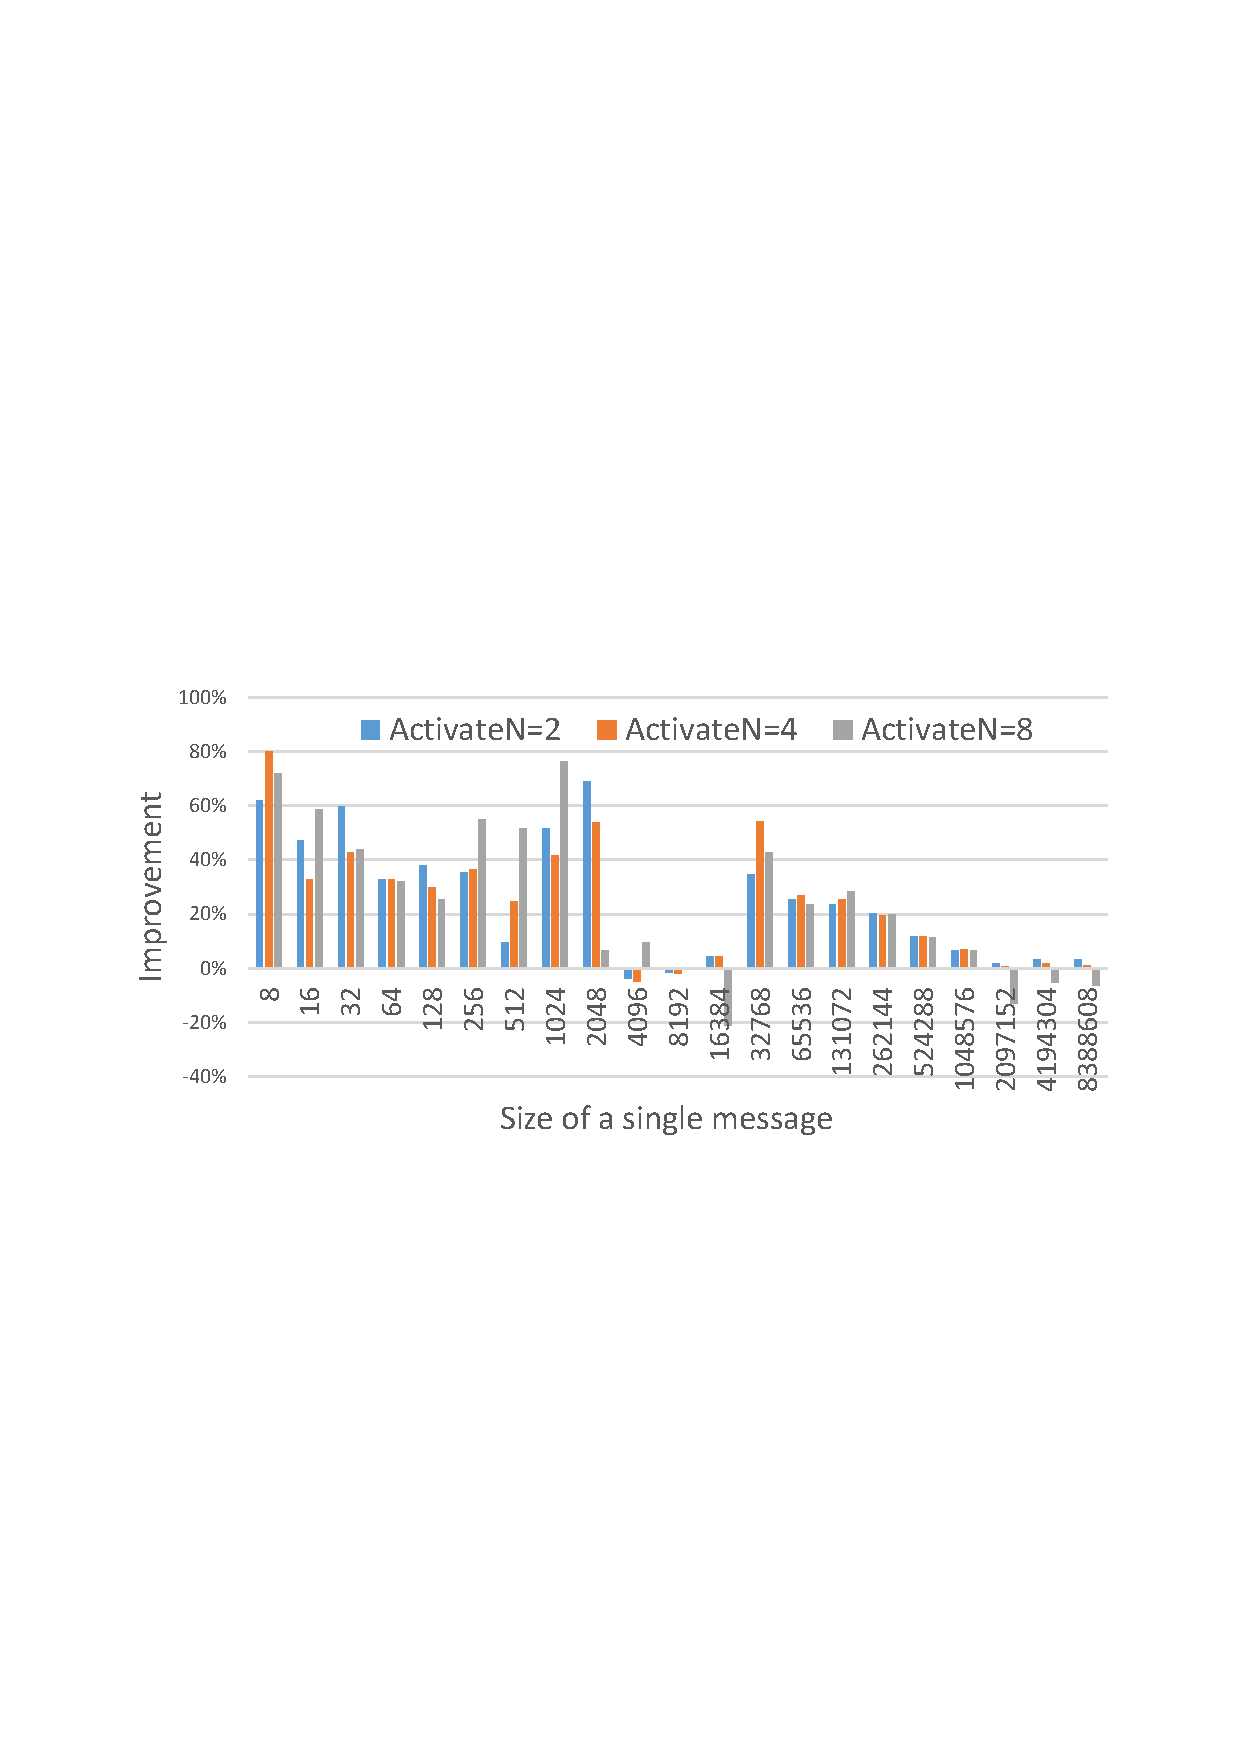
\includegraphics[width=0.49\textwidth]{./Figures/hpcd/Multi-port-p2p.pdf}}
  \caption{Multiple endpoints delivery throughput compared to single endpoints.}
	\label{Multi-port}
	\vspace{0.2in}
\end{figure*}

Besides, as the intra-node communication can be overlappable with inter-node communication, gathering/scattering overhead can be overlapped with inter-node overhead.

Although there are a lot of parallelism, there is no method using all these parallelism to optimize the communication performance of all-to-all.
